\documentclass[aspectratio=169,10pt]{beamer}
\usetheme{Madrid}
\usepackage{graphicx}
\usepackage{amssymb}

% Tắt hiệu ứng shadow để giao diện phẳng, sắc nét
\setbeamertemplate{blocks}[rounded][shadow=false]
\setbeamertemplate{navigation symbols}{}

% Color configuration
\definecolor{primaryblue}{RGB}{20, 55, 110}
\setbeamercolor{palette primary}{bg=primaryblue,fg=white}
\setbeamercolor{structure}{fg=primaryblue}

\begin{document}

\begin{frame}{Graph of a Two-Variable Function}
    \begin{columns}[T]
        % Cột trái (56%): Nội dung câu hỏi và định nghĩa Level Curves
        \begin{column}{0.56\textwidth}
            \begin{block}{Question: How can we plot a surface?}
                \small
                \begin{itemize}
                    \item For $s = g(t)$, we pick points $t_1, \dots, t_n$ and connect points with a smooth curve.
                    \item For $z = f(x, y)$, this method fails. Instead:
                    \begin{itemize}
                        \item For each $z = z_0$, draw the \textbf{level curve} $z_0 = f(x, y)$.
                        \item This is the \textbf{intersection} of the surface $z = f(x, y)$ and the horizontal plane $z = z_0$:
                        \[
                            L_{z_0} := \{(x, y) \mid f(x, y) = z_0\}.
                        \]
                    \end{itemize}
                \end{itemize}
            \end{block}
        \end{column}

        % Cột phải (42%): Animation Manim 3D cắt và chiếu đường mức xuống Oxy
        \begin{column}{0.42\textwidth}
            \centering
            \vspace{0.15cm}
            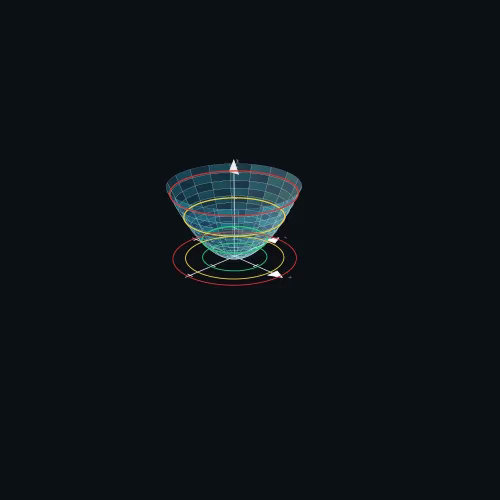
\includegraphics[width=0.92\linewidth, keepaspectratio]{ContourProjectionScene.png}
            
            \vspace{0.1cm}
            {\tiny \textcolor{gray}{\textit{Slicing at $z = z_0$ and projecting contours to the $xy$-plane}}}
        \end{column}
    \end{columns}
\end{frame}

\end{document}
